% !TeX spellcheck = fr_FR
\documentclass{beamer}
\setbeamercolor{background canvas}{bg=white}

\usetheme{metropolis}
\metroset{sectionpage=none,progressbar=frametitle}

\usepackage{appendixnumberbeamer}
\usepackage{polyglossia}
\setdefaultlanguage{french}
\usepackage{mathtools,amsfonts,amssymb}
\usepackage{booktabs}
\usepackage{enumitem}

\usepackage{subfiles}

\usepackage{csquotes}
\usepackage[
	backend=biber,
	sorting=nyt,
	style=authoryear,
	citestyle=authoryear
]{biblatex}
\addbibresource{../rapport/references.bib}

\usepackage{dsfont}
\usepackage{stmaryrd}
\usepackage{graphicx}
\usepackage{subcaption}
\usepackage{siunitx}

\usepackage{hyperref}
\usepackage{cleveref}

\newcommand{\RR}{\mathbb{R}}
\newcommand{\NN}{\mathbb{N}}
\newcommand{\ZZ}{\mathbb{Z}}
\newcommand{\PP}{\mathbb{P}}
\newcommand{\EE}{\mathbb{E}}
\newcommand{\Var}{\mathrm{Var}}

\DeclareMathOperator*{\argmax}{argmax} % no space, limits underneath in displays

\title{
	\textit{Processus ponctuels et réseaux de neurones récurrents}
}
\author{
	Cheikh Fall\\
	Wilson Jallet
}

\date{11 décembre 2018}

\begin{document}
\maketitle

\begin{frame}{Introduction}
Beaucoup de phénomènes se manifestent par des événements ponctuels.\pause

L'arrivée de certains événements peut favoriser l'arrivée d'autres dans le futur.
\end{frame}

\subfile{models.tex}

\begin{frame}{Apprentissage}
Maximiser la fonction de log-vraisemblance
\begin{equation}\label{eq:logLikelihood}
\begin{aligned}
\ell &= P\left( \{(t_i,k_i)\}_i \mid \Theta \right) \\
&= \sum_{i=1}^{I}\log \lambda^{k_i}_{t_i} - \int_0^T \bar{\lambda}_t\,dt.
\end{aligned}
\end{equation}
avec $\bar{\lambda}_t = \sum_k \lambda^k_t$ l'intensité totale.

\textbf{Remarque} Difficile à calculer!
\end{frame}

\begin{frame}{Prédiction}
On donne un début de séquence $(t_1,k_1)\ldots (t_{i-1}, k_{i-1})$ au réseau pour générer les paramètres pour $(t_{i-1}, t_i]$.
\begin{itemize}
	\item[$\rightarrow$] On peut calculer $\lambda_t = f(t\mid\mathcal{F}_{t_{i-1}})$ pour $t\geq t_{i-1}$
	\item[$\rightarrow$] Permet d'estimer le prochain événement $(t_i, k_i)$
	\[
	\begin{aligned}
		\hat{t}_i &= \EE\left[t_i \middle| \mathcal{F}_{t_{i-1}}\right] \\
		\hat{k}_i &= \argmax_{k}\EE\left[\lambda^k_t/\bar{\lambda}_t\middle| \mathcal{F}_{t_{i-1}} \right]
	\end{aligned}
	\]
\end{itemize}
\end{frame}

\section{Expériences}

\subsection{Hawkes symétrique}

\begin{frame}{Expériences}
Dans le rapport $\rightarrow$ difficultés à apprendre des processus au moins multivariés $K\geq 2$.\pause

$\rightarrow$ Erratum dans le calcul de la vraisemblance (corrigé)

\textbf{Expérience 1} Processus de Hawkes bivarié symétrique (noyau exponentiel) sur $[0, 3600]$
\begin{itemize}
	\item $\alpha = \begin{bmatrix}0.1 & 0.01 \\ 0.01 & 0.1\end{bmatrix}$
	\item $\beta = 1$
	\item $\mu_1 = \mu_2 = \num{0.1}$
\end{itemize}
\end{frame}

\begin{frame}

\begin{figure}
	\includegraphics[width=\linewidth]{../results/intensity_baseHawkes2D.pdf}
	\caption{Intensité du processus de Hawkes, généré avec \texttt{tick}.}
\end{figure}
\end{frame}

\begin{frame}
\begin{figure}
	\begin{subfigure}{\linewidth}
		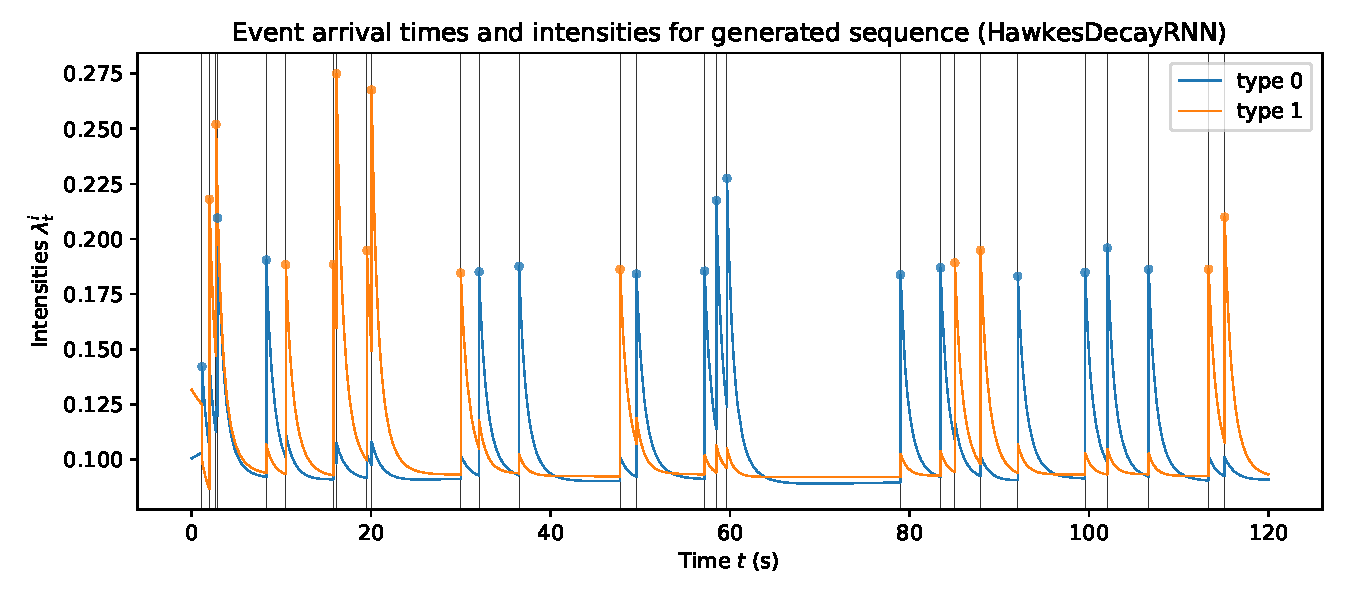
\includegraphics[width=\linewidth]{../results/intensity_HawkesDecayRNN_2d_hidden128_20181209-132014.pdf}
		\caption{Intensité et événements générés par le Decay-RNN calibré sur le Hawkes bivarié.}
	\end{subfigure}
	\caption{Intensité apprise par le réseau RNN.}
\end{figure}
\end{frame}

\begin{frame}
\begin{figure}\ContinuedFloat
\begin{subfigure}{\linewidth}
	\includegraphics[width=\linewidth]{../results/intensity_HawkesDecayRNN_2d_hidden64_20181209-003122_OLD.pdf}
	\caption{Avec une erreur d'indice dans le calcul. Le réseau apprend à <<~écraser~>> les autres composantes de l'intensité après chaque événement.}
\end{subfigure}
\end{figure}
\end{frame}

\begin{frame}
\begin{figure}
	\centering
	\includegraphics[width=\linewidth]{../results/2D_Hawkes_Data_RMSE_20181209-181315.pdf}
	\caption{Résultats pour la prédiction d'événements, apprentissage sur des trajectoires d'un Hawkes bivarié ($K=2$).}
\end{figure}
\end{frame}

\begin{frame}
\begin{figure}
	\begin{subfigure}{\linewidth}
		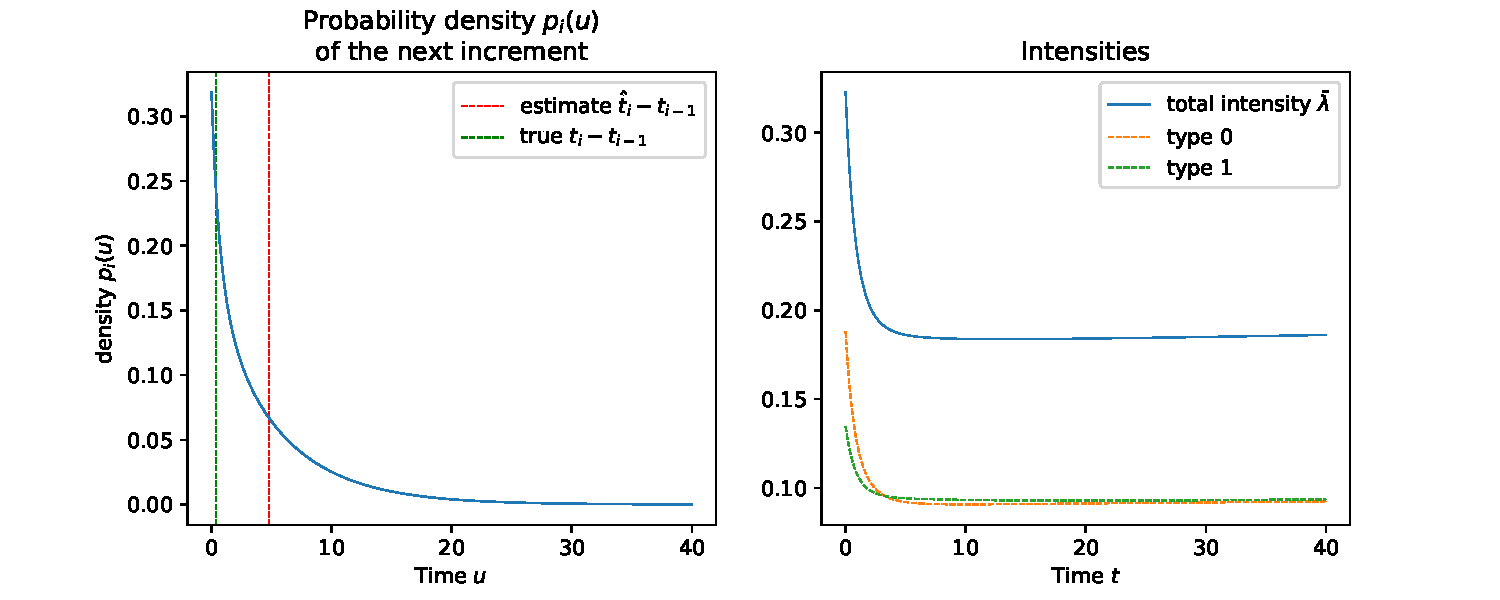
\includegraphics[width=\linewidth]{../notebooks/decayrnn_2d_prediction_graphs_hidden128_NEW.pdf}
		\caption{Le processus de Hawkes sous-jacent est symétrique: pour le prochain événement, les types sont équiprobables.}
	\end{subfigure}
	\caption{Loi du temps du prochain événement, et intensités $(\lambda^i_t)_{t\geq t_{i-1}}$ de chaque type.}
\end{figure}
\end{frame}

\begin{frame}
\begin{figure}\ContinuedFloat
	\begin{subfigure}{\linewidth}
		\includegraphics[width=\linewidth]{../notebooks/decayrnn_2d_prediction_graphs_OLD.pdf}
		\caption{Avec la faute de calcul. Le type du prochain événement est certainement celui du dernier.}
	\end{subfigure}
\end{figure}
\end{frame}

\subsection{Hawkes asymétrique}

\begin{frame}
\textbf{Expérience 2} Processus de Hawkes asymétrique, $T = 1800$
\begin{itemize}
	\item $\alpha = \begin{bmatrix}0.1 & 0.07\\ 0.01 & 0.15\end{bmatrix}$
	\item $\beta = 1$
	\item $\mu_1 = \num{0.3} = 3\mu_2$
\end{itemize}
\end{frame}

\begin{frame}
\begin{figure}
	\includegraphics[width=\linewidth]{../results/intensity_baseHawkes2D_asymmetrical.pdf}
	\caption{Intensité du processus généré avec \texttt{tick}.}
\end{figure}
\end{frame}

\begin{frame}
\begin{figure}
	\includegraphics[width=\linewidth]{../results/intensity_HawkesDecayRNN_2d_hidden128_20181209-212603.pdf}
	\caption{Trajectoire générée par le Decay-RNN calibré sur le processus asymétrique.}	
\end{figure}
\end{frame}

\begin{frame}
\begin{figure}
	\includegraphics[width=\linewidth]{../results/intensity_HawkesLSTM_2d_hidden128_20181209-214506.pdf}
	\caption{Trajectoire générée par le LSTM.}
\end{figure}
\end{frame}

\begin{frame}
\begin{figure}
	\includegraphics[width=\linewidth]{../results/2D_Hawkes_Asymmetrical_Data_RMSE_20181209-221850.pdf}
	\caption{Résultats pour la prédiction d'événements, sur les données Hawkes asymétrique.}
\end{figure}
\end{frame}

\section{Conclusion}

\begin{frame}[t,allowframebreaks]{References}
	\printbibliography
\end{frame}

\end{document}
